
\section{Methods}

This study employed a custom, iterative methodology to investigate and develop an activity-monitoring system for the Reachy Mini. The approach shares similarities with the Design Science Research (DSR) framework, which is suitable for design-oriented research involving the development and evaluation of an artefact \cite{hevner2007}. The approach was selected because the technical feasibility of the system was initially uncertain and several technical choices required investigation before implementation.

The methodology consisted of five phases:

\begin{enumerate}
    \item Research: identifying stakeholder needs, establishing requirements, and investigating existing techniques.
    \item Design: selecting suitable models and defining the technical architecture.
    \item Realisation: implementing the activity-recognition pipeline and integrating it with the robot.
    \item Testing: evaluating model performance and system behaviour under different conditions.
    \item Evaluation: assessing feasibility, identifying limitations, and formulating recommendations.
\end{enumerate}

The phases were not strictly sequential. Research informed design decisions, while implementation and testing were conducted iteratively. Results from experiments were used to refine technical choices and improve the artefact. This approach supported early validation and incremental improvement, which suited the exploratory nature of the project \cite{geeksforgeeks2025}. A traditional waterfall approach was considered less suitable because the technical choices were not fully determined at the start and the project required opportunities to incorporate findings during implementation \cite{agilescrumgroup}.

Figure~\ref{fig:prototyping-approach} illustrates the iterative prototyping approach. Figure~\ref{fig:research-approach} shows the activities conducted during the research phase.

\begin{figure}[htbp]
    \centering
    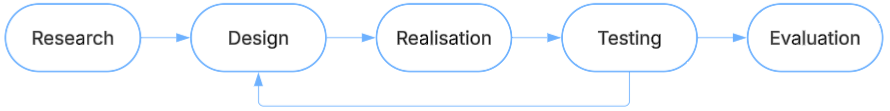
\includegraphics[width=0.9\linewidth]{figures/prototyping-approach.png}
    \caption{Iterative prototyping approach used in the project.}
    \label{fig:prototyping-approach}
\end{figure}

\subsection{Requirements and software requirements specification}

The research began with a stakeholder analysis to identify the parties involved and their interests and needs. Functional and non-functional requirements were derived from the project description and meetings with the client. These requirements were consolidated in a software requirements specification (SRS), which served as the reference for design and evaluation.

The functional requirements cover perception and local processing, robot behaviour and interaction, activity and exercise recognition, assessment and feedback, and session management. The non-functional requirements address privacy, recognition accuracy, reliability, usability, and safety. The complete SRS contains the detailed requirement statements and is included as an attachment to the article.

The research was organised around two complementary activities. First, existing techniques for person detection, pose estimation, and activity recognition were investigated. Second, relevant scientific literature, datasets, standards, and guidelines were studied to identify suitable approaches and relevant constraints. The findings were compared against the system requirements and the Reachy Mini's camera and computational capabilities. This process informed the selection of candidate models and the subsequent evaluation of their suitability.

\begin{figure}[htbp]
    \centering
    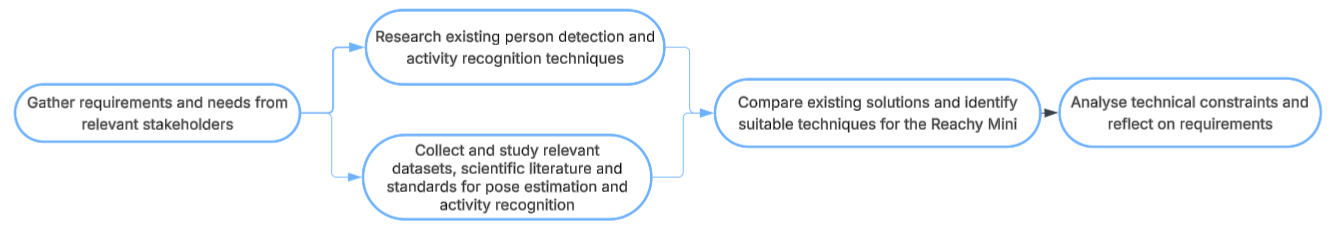
\includegraphics[width=0.9\linewidth]{figures/research-approach.png}
    \caption{Research activities used to establish requirements and identify suitable techniques for the Reachy Mini.}
    \label{fig:research-approach}
\end{figure}

\subsection{Pose-model research and selection}

Candidate models for human pose detection and temporal activity analysis were investigated under the Reachy Mini's CPU and camera constraints. The candidates included BlazePose for fast 2D pose detection, ViTPose as a transformer-based 2D estimator, WHAM and CameraHMR for 3D motion or pose-and-shape estimation, MoveNet for lightweight 2D pose estimation, SAM2 for segmentation, PySlowFast for video classification, FSPose for fused-heatmap pose estimation, GraphEnet for graph-based pose estimation, YOLOPose for pose estimation using the YOLO framework, MoViNets for efficient video recognition, and TSM-MobileNetV2 for lightweight temporal modelling.

BlazePose, MoViNet-A0, TSM-MobileNetV2, ViTPose, YOLOPose, and MoveNet were benchmarked under comparable conditions. Throughput and mean pose-inference time were recorded. The evaluation also considered whether each model could run on the robot and produce the COCO-17 keypoint representation required by the downstream feature-extraction and recognition pipeline.

MoveNet Lightning int8, executed through LiteRT, was selected because it provided the most suitable trade-off between speed, keypoint compatibility, and deployment feasibility.

\subsection{Training, export, and inference}

No new video recordings were collected for model training. Instead, the recognition models were trained using existing COCO-17 skeleton data published by OpenMMLab for NTU RGB+D 60 \cite{shahroudy2016ntu} (wave and clapping) and UCF101 \cite{soomro2012ucf101} (pushup, squat, and jumping jacks). HMDB51 was used only as an external test set. All other dataset classes were labelled as none.

Each clip was resampled from 30 to approximately 10 FPS to match the robot camera. The clips were then divided into temporal windows using the same feature-extraction code as the live system: 1.5-second windows with nine features for the binary wave model, and 3-second windows with 34 features for the six-class action model. To approximate the table-mounted camera perspective, each clip was also windowed with leg and hip keypoints removed.

Random forests were trained using scikit-learn \cite{pedregosa2011scikit}. The wave model used 100 trees with a maximum depth of six, while the action model used 300 class-balanced trees. The models were evaluated using five-fold GroupKFold by subject or footage group, following \cite{saeb2017need}. Precision, recall, and F1 scores were calculated from out-of-fold predictions. A confidence threshold was tuned for each class using these predictions; windows below the threshold were classified as none.

The final forests were fitted on all training windows and exported to compressed \texttt{.npz} files containing the decision-tree node arrays. On the robot, a NumPy-only implementation traverses these trees and reproduces scikit-learn's \texttt{predict\_proba} behaviour, removing the need for scikit-learn during inference.

\subsection{Robot integration}

The applications use the Reachy Mini Python SDK (\texttt{reachy\_mini} 1.10.0, matched to the daemon version) for motion and the daemon REST API on port 8000 for state management.

Before camera, tracking, or movement operations, a standard-library preflight procedure checks network reachability, daemon and backend state, running applications and movements, motor mode, sleep pose, camera ownership, and tracker frames. When automatic correction is enabled, the procedure enables the motors, executes the wake-up movement, and reacquires the camera. It returns an explicit ready, not-ready, or unreachable status. A context manager combines preflight checks, SDK connection, and cleanup, including stopping head tracking and optionally returning the robot to its sleep pose.

Because the vision loop operates at approximately 10 FPS while the daemon controls the robot at 50 Hz, a dedicated thread streams \texttt{set\_target} commands at 50 Hz. Each recognised action produces a distinct antenna movement pattern defined by amplitude, frequency, and a whole number of cycles ending at the neutral pose. Head and body following use an integrating controller based on the image-position error of the torso centre. Body yaw extends the tracking range beyond the head's 60-degree movement limit relative to the body.

Additional integrations include an annotated MJPEG camera stream for browser-based observation without a local display, a remote-inference mode that sends low-resolution frames (192$\times$108 pixels) to a laptop GPU and receives keypoints over HTTP, and a coach workflow for training personalised models on the robot's CPU. In the coach workflow, scikit-learn runs in a low-priority subprocess to keep the camera and tracking loops responsive. A failed training run does not overwrite the previous model. Deployment uses an isolated virtual environment to avoid modifying the robot's system environment.

\subsection{Testing and evaluation}

Testing and evaluation examined the technical feasibility of the system against the requirements established during the research phase. Model performance was assessed using the benchmark results and the out-of-fold precision, recall, and F1 scores. HMDB51 provided an external test set beyond the datasets used for training. Camera-framing experiments considered the effect of removing hip and leg keypoints on the information available for activity recognition.

The evaluation also considered inference speed, CPU-only deployment, compatibility with the Reachy Mini's camera and movement interfaces, and system responsiveness during simultaneous recognition and tracking. The findings were used to identify technical limitations and formulate recommendations for further development. The project focused on technical feasibility; it did not validate a clinical assessment instrument or establish clinical suitability for physiotherapy.

\newpage